\documentclass[a4paper,12pt]{report}
\usepackage[utf8]{inputenc}
\usepackage{amsmath}
\usepackage{graphicx}
\usepackage{listings}
\usepackage{tikz}
\usepackage[T1]{fontenc}
\usepackage{color}
\usetikzlibrary{arrows,automata}
\definecolor{pythonred}{rgb}{0.6,0,0} % for strings
\definecolor{pythongreen}{rgb}{0.25,0.5,0.35} % comments
\definecolor{pythonpurple}{rgb}{0.5,0,0.35} % keywords
	\definecolor{pythondocblue}{rgb}{0.25,0.35,0.75} % javadoc
	 
	\lstset{language=python,
	basicstyle=\ttfamily,
	keywordstyle=\color{pythonpurple}\bfseries,
	stringstyle=\color{pythonred},
	commentstyle=\color{pythongreen},
	morecomment=[s][\color{pythondocblue}]{/**}{*/},
	numbers=left,
	numberstyle=\tiny\color{black},
        stepnumber=2,
	numbersep=10pt,
	tabsize=4,
	showspaces=false,
	showstringspaces=false}

% Title Page

 \title{\bfseries\huge \textcolor{purple}{\underline {EEP-703 Computer Network Lab}} \\{\textcolor{blue}{Assignment 9-Capturing and analyzing network traffic
using Wireshark Tool}}}
\author{\bfseries\large\textcolor{black}  {Harshit Kumar Gupta}\\ {\textcolor{black} {2013EET2369 }}\\

\includegraphics[width=3cm,height=3.4cm]{./iit.png}\\\noindent Computer Technology\\
\noindent Department Of Electrical Engineering\\IIT DELHI}
% iit.png: 282x282 pixel, 72dpi, 9.95x9.95 cm, bb=0 0 282 282
\begin{document}
\maketitle
\tableofcontents



\chapter{\textcolor{blue}{\underline {PROBLEM STATEMENT}}}
\noindent 
Networks need watching, or network administration, observe network traffic on a real­time basis using (also called 
sniffing)  protocol analysis tools such as wireshark.
 Now, you are given the following tasks:
  \begin{enumerate}

\item List the different protocols you encounter when you visit a page (www.example.com) and 
explain their significance. Every URL you visit is hosted on a certain server having an IP 
address. Find out the IP addresses corresponding to URL you visited and your machine.
\item  Open the first packet which has the IP addresses of www.example.com in the 
destination and has HTTP as the protocol.
\begin{enumerate}
 \item  Explain the five major headings: Frame, Ethernet Protocol, IPv4, TCP and HTTP. 
Why these different protocols are involved in the same message? How are these 
protocols related? 
\item Using wireshark, observe normal network traffic. Can you separately see TCP/IP traffic, 
    IPX traffic and NETBEUI traffic? What is the meaning of these different types of traffic?
\item Does the information in this packet state about the browser and OS you are 
using?  Does it show that you are sending a cookie? 
\end{enumerate}

\end{enumerate}


\begin{center}
\chapter{\textcolor{blue}{\underline {ABSTRACT}}}
\end{center}
\begin{enumerate}
 


\item The whole problem is to understand the Wireshark tools  
\item Main Objective is to understand working of varios protocols. 
\item Learnig how to capture network traffic.

\end{enumerate}
\begin{center}
\chapter{\textcolor{blue}{\underline {INTRODUCTION}}}
\end{center}
\noindent \textbf Wireshark is a free and open-source packet analyzer. It is used for network troubleshooting, analysis, software and communications protocol development, and education.
Wireshark is cross-platform, using the GTK+ widget toolkit in current releases, and Qt in the development version, to implement its user interface, and using pcap to capture packets.\\

Wireshark is very similar to tcpdump, but has a graphical front-end, plus some integrated sorting and filtering options.

Wireshark allows the user to put network interface controllers that support promiscuous mode into that mode, in order to see all traffic visible on that interface, not just traffic addressed to one of the interface's configured addresses and broadcast/multicast traffic.
\begin{center}
\chapter{\textcolor{blue}{\underline {SPECIFICATIONS AND ASSUMPTIONS}}}
\end{center}
\section*{Specifications}
\begin{enumerate}
 
\item Data can be captured "from the wire" from a live network connection or read from a file of already-captured packets..
\item Live data can be read from a number of types of network, including Ethernet, IEEE 802.11, PPP, and loopback.

\item Captured network data can be browsed via a GUI, or via the terminal (command line) version of the utility, TShark


\end{enumerate}

\section*{Assumptions}
\begin{enumerate}
\item Data display can be refined using a display filter.
\item Wireshark  put wireless network interface controllers into monitor mode.

\end{enumerate}
 
\begin{center}
\chapter{\textcolor{blue}{\underline {LOGIC USED/METHODOLOGY}}}
\end{center}
The methodology that is used for developing this project work is defined below:
\begin{enumerate} 
\item After downloading and installing Wireshark, you can launch it and click the name of an interface under Interface List to start capturing packets on that interface. For example, if you want to capture traffic on the wireless network, click your wireless interface. You can configure advanced features by clicking Capture Options, but this isn’t necessary for now.
\item As soon as you click the interface’s name, you’ll see the packets start to appear in real time. Wireshark captures each packet sent to or from your system. If you’re capturing on a wireless interface and have promiscuous mode enabled in your capture options, you’ll also see other the other packets on the network.
\item Click the stop capture button near the top left corner of the window when you want to stop capturing traffic.

\end{enumerate}
\begin{center}
\chapter{\textcolor{blue}{\underline {EXECUTION DIRECTIVES}}}\end{center}
\begin{enumerate}
 \item  Filtering Packets---

If you’re trying to inspect something specific, such as the traffic a program sends when phoning home, it helps to close down all other applications using the network so you can narrow down the traffic. Still, you’ll likely have a large amount of packets to sift through. That’s where Wireshark’s filters come in.

\item The most basic way to apply a filter is by typing it into the filter box at the top of the window and clicking Apply (or pressing Enter). For example, type “dns” and you’ll see only DNS packets. When you start typing, Wireshark will help you autocomplete your filter.



\end{enumerate}
\begin{center}
\chapter{\textcolor{blue}{\underline {RESULTS AND CONCLUSIONS}}}\end{center}

\begin{center}
 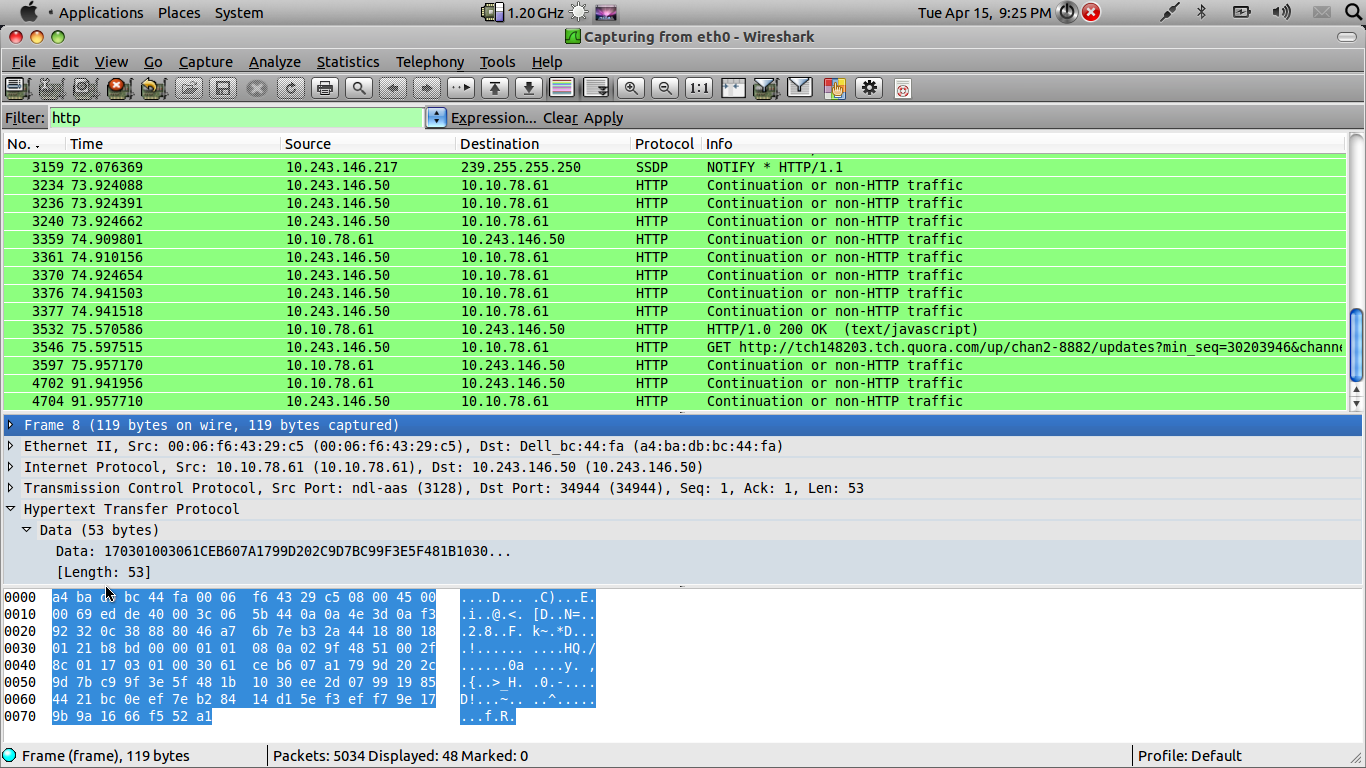
\includegraphics[width=13 cm,height=12 cm]{./Screenshot-1.png}
Capturing and analyzing network traffic using Wireshark
\end{center}
\begin{center}
 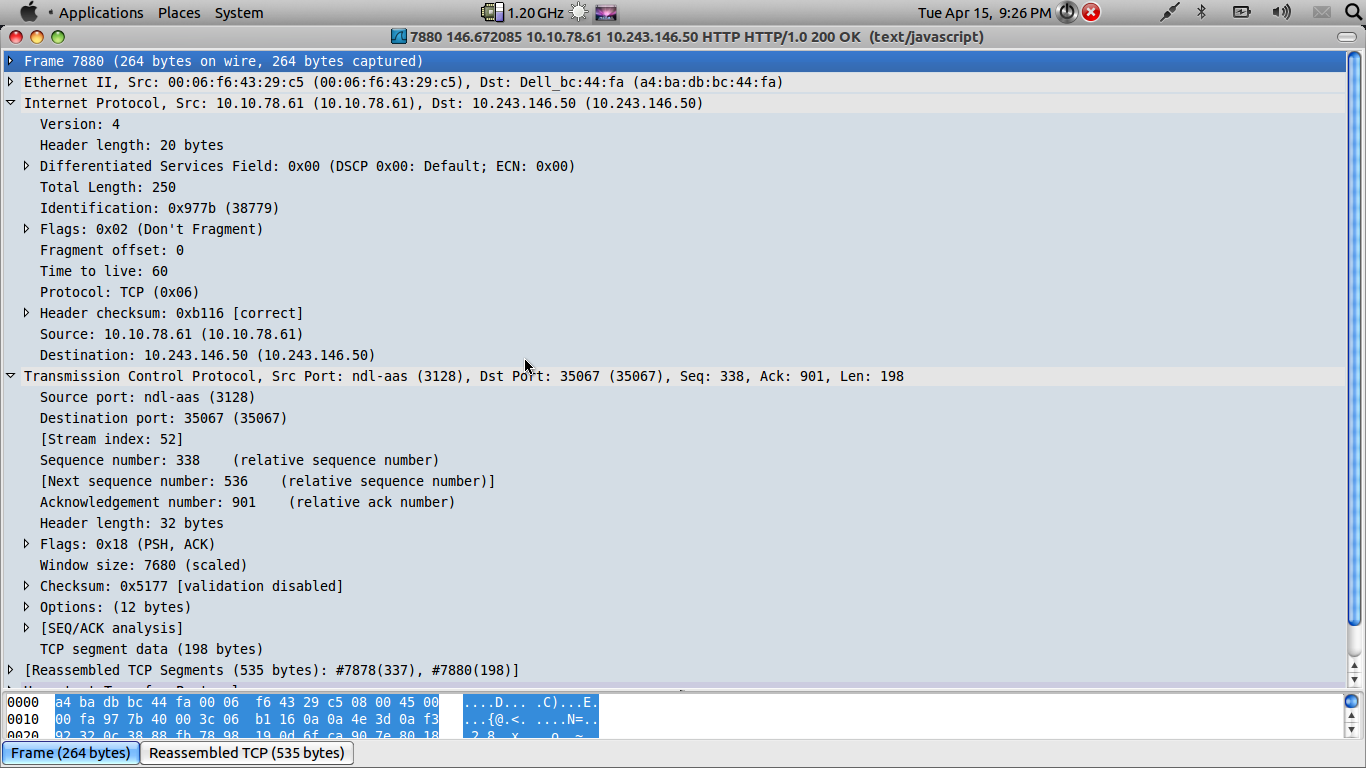
\includegraphics[width=13 cm,height=12 cm]{./Screenshot-2.png}
Analysis of various packet Headers using Wireshark
\end{center}
\begin{center}
 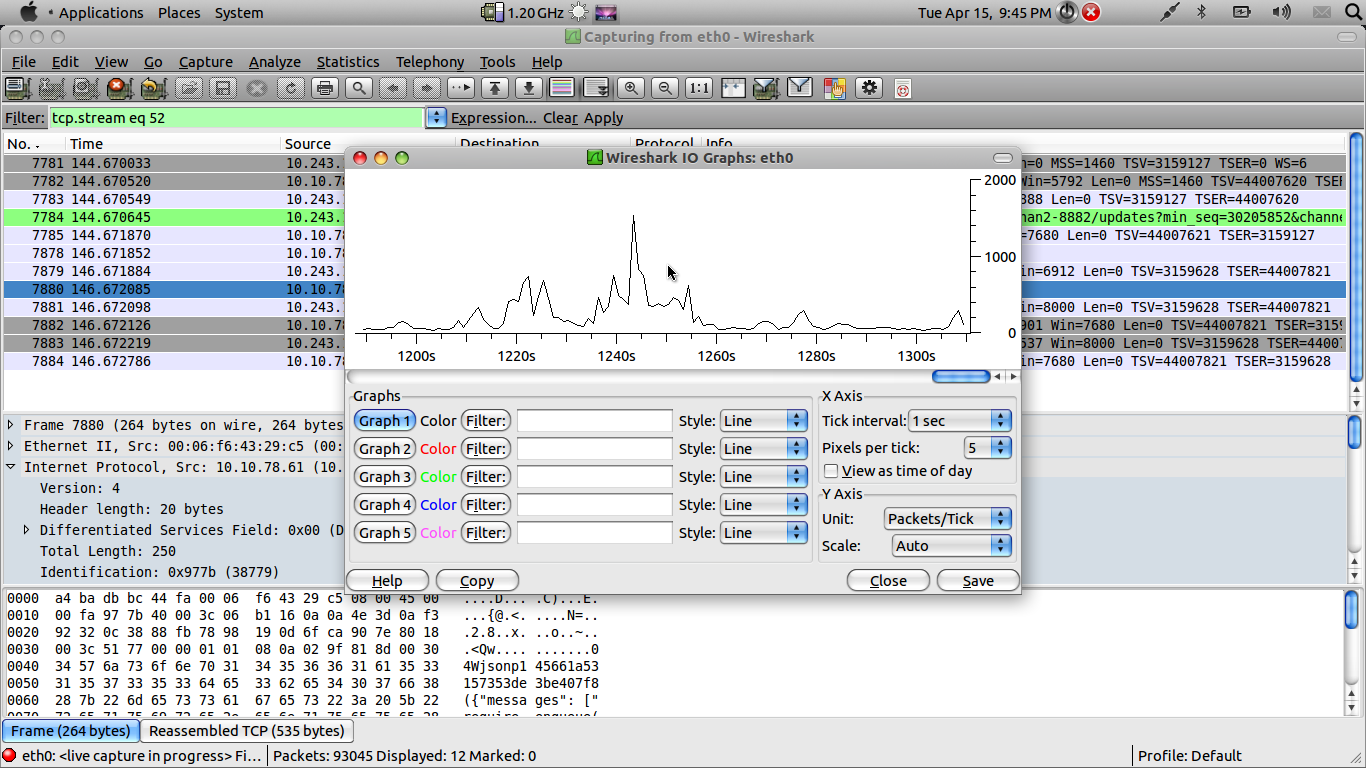
\includegraphics[width=13 cm,height=12 cm]{./Screenshot-5.png}
Analysis of IO using  Wireshark (IO graph)
\end{center}
\begin{center}
 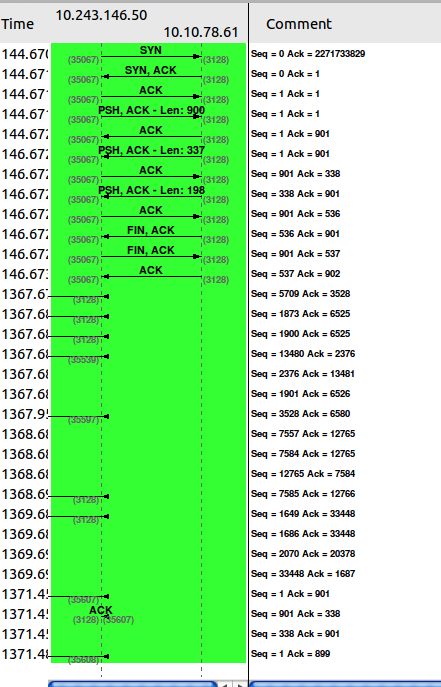
\includegraphics[width=13 cm,height=12 cm]{./Screenshot-6.png}
TCP packets transfer analysis
\end{center}
\begin{center}


 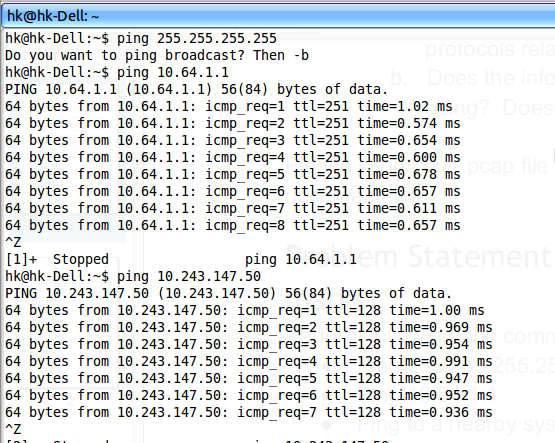
\includegraphics[width=13 cm,height=12 cm]{./Screenshot-3.png}
Ping 255.255.255.255 , 10.64.1.1 and  a nearby system 
\end{center}
\begin{center}


 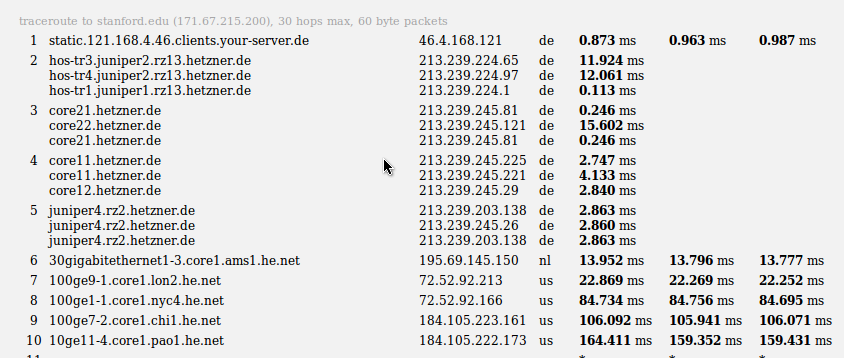
\includegraphics[width=13 cm,height=12 cm]{./Screenshot-4.png}
Trace the route to http://www.stanford.edu/  using traceroute
\end{center}

\end{document}  